% main.tex
% Fichero principal de transparencias (incluye a todos los demás).

% Compilar a .pdf con LaTeX (pdflatex)
% Es necesario instalar Beamer (paquete latex-beamer en Debian)
%

% Gráficos:
% Los gráficos pueden suministrarse en PNG, JPG, TIF, PDF, MPS
% Los EPS deben convertirse a PDF (usar epstopdf)
%
\documentclass[17pt,aspectratio=169,hyperref=pdfusetitle]{beamer}
\usetheme[orchid]{Hannover}
\beamertemplatenavigationsymbolsempty
\setbeamertemplate{headline}{}
\useoutertheme{infolines}

\usepackage[spanish]{babel}
\usepackage[utf8]{inputenc}
\usepackage{graphics}
%\usepackage{amssymb} % Simbolos matematicos
%\usepackage[pdfusetitle]{hyperref}

\usepackage{chronosys}

%% two slides per page
%\usepackage{pgfpages}
%\pgfpagesuselayout{2 on 1}[a4paper,border shrink=5mm]

\newcommand\YUGE{\fontsize{48}{60}\selectfont}

\newcommand{\secimage}{figs/bookpages}
\AtBeginSection[]
{
  {
    \usebackgroundtemplate{\includegraphics[width=\paperwidth,height=\paperheight]{\secimage}}
    \begin{frame}<beamer>

      \begin{center}
        {\YUGE\bf\insertsection}
      \end{center}
    \end{frame}
  }
  \renewcommand{\secimage}{figs/bookpages}
}


\title[Spinning out Bitergia]{Challenges and Learnings \\
  from spinning out Bitergia from the university}
%\subtitle{}
\author[Jesus M. Gonzalez-Barahona]{Jesus M. Gonzalez-Barahona}
\institute[URJC]{Universidad Rey Juan Carlos \\
  @jgbarah ~~~~~ \url{http://github.com/jgbarah/presentations}}

\date[]{Madrid (Spain), September 16th 2019}

\begin{document}

%\begin{frame}[label=firstframe]
\begin{frame}
  \maketitle
\end{frame}


\begin{frame}

  {\em
    \begin{center}
      %\begin{quote}
      Chance is important \\
      but then you have to work...\\
      %\end{quote}
    \end{center}
  }
\end{frame}


%%%%%%%%%%%%%%%%%%%%%%%%%%%%%%%%%%%%%%%%%%%%%%%%%%%%%%%%%%%%%%%%
%%%%%%%%%%%%%%%%%%%%%%%%%%%%%%%%%%%%%%%%%%%%%%%%%%%%%%%%%%%%%%%%
% lista de temas                                               %
%%%%%%%%%%%%%%%%%%%%%%%%%%%%%%%%%%%%%%%%%%%%%%%%%%%%%%%%%%%%%%%%
%%%%%%%%%%%%%%%%%%%%%%%%%%%%%%%%%%%%%%%%%%%%%%%%%%%%%%%%%%%%%%%%


\definecolor{lightviolet}{HTML}{F4AFF4}
\definecolor{lightorange}{HTML}{FFA17F}
\definecolor{lightgreen}{HTML}{98FB98}
\definecolor{lightred}{HTML}{FF5C5C}
\definecolor{lightblue}{HTML}{89AFCF}
\definecolor{lightbrown}{HTML}{B58868}

%%-----------------------------------------
%%-----------------------------------------
\section{Some context}



%%-----------------------------------------
\begin{frame}[fragile]
  \frametitle{The team is important}

  \begin{center}
  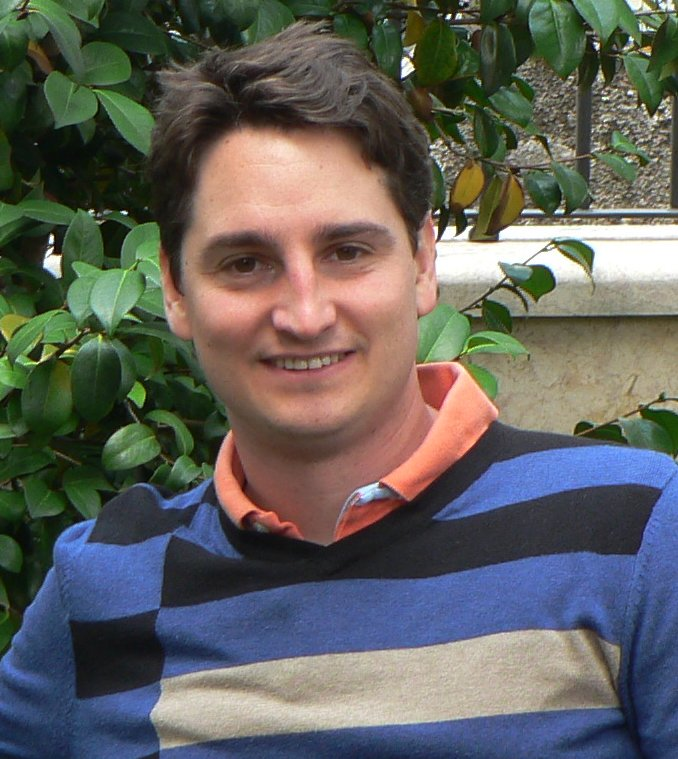
\includegraphics[height=4.5cm]{figs/gregorio-robles}
  
\includegraphics[height=4.5cm]{figs/libresoft}
  \end{center}  
  
\end{frame}

%%-----------------------------------------
\begin{frame}[fragile]
  \frametitle{The team is important}

  Having great people around is very important \\
  Playing in a team is much more fun \\
  Together you can reach further \\
  
  \begin{center}
    We had the chance of trying it
  \end{center}  
  
\end{frame}


%%-----------------------------------------
\begin{frame}[fragile]
  \frametitle{We had some principles}

  The importance of sharing \\
  The importance of ethics \\
  The importance of tools \\

  \begin{center}
    We were lucky this worked
  \end{center}
\end{frame}


%%-----------------------------------------
\begin{frame}[fragile]
  \frametitle{The starting point (2000-2001)}

  \begin{center}
  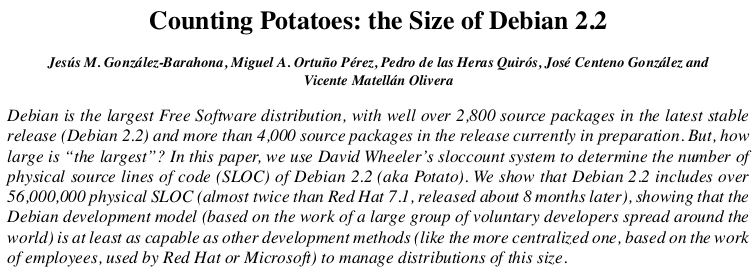
\includegraphics[width=12cm]{figs/counting-potatos}

  
\includegraphics[width=6cm]{figs/upgrade}
  \end{center}  
  
\end{frame}

%%-----------------------------------------
\begin{frame}[fragile]
  \frametitle{Counting potatoes}

  Any detail may change a life \\
  In some moments you're ready for a change \\
  and you feel you have been preparing for it \\
  
  \begin{center}
    Switching fields may be rebooting from scratch
  \end{center}
  
\end{frame}

%%-----------------------------------------
\begin{frame}[fragile]
  \frametitle{Becoming ``academic'' (2001-2003)}

  \begin{center}
  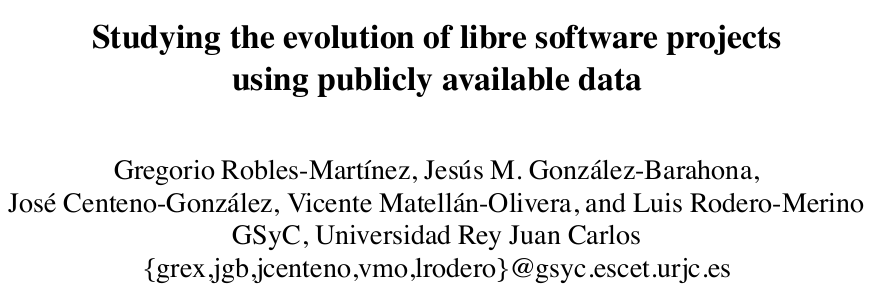
\includegraphics[width=12cm]{figs/evolution-data}
  \end{center}  
  
\end{frame}

%%-----------------------------------------
\begin{frame}[fragile]
  \frametitle{Entering mainstream}

  The are niches of opportunity \\
  that you can exploit better than others \\
  but quickly you need to learn new stuff \\
  
  \begin{center}
    Starting in a new research field \\
    is not always easy \\
  \end{center}  
  
\end{frame}


%%-----------------------------------------
\begin{frame}[fragile]
  \frametitle{Building tools (2002-2015)}

  \begin{center}
  
\includegraphics[width=12cm]{figs/cvsanaly}
  \end{center}  
  
\end{frame}

%%-----------------------------------------
\begin{frame}[fragile]
  \frametitle{Tools \& research}

  Tools are important and cool \\
  Tools help you learn the details \\
  Tools can be done in collaboration \\
  
  \begin{center}
      Good tools don't guarantee publication
  \end{center}  
  
\end{frame}


%%-----------------------------------------
\begin{frame}[fragile]
  \frametitle{Benefiting from expertise (2005-2008)}

  \begin{center}
  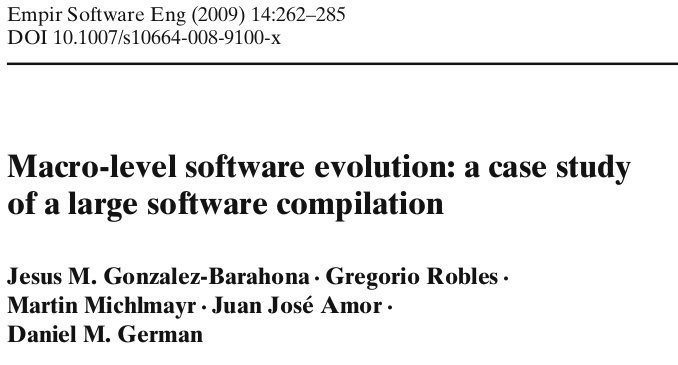
\includegraphics[width=12cm]{figs/macro-evolution}
  \end{center}  
  
\end{frame}

%%-----------------------------------------
\begin{frame}[fragile]
  \frametitle{The need of patience}

  A solid work may take a little while... \\
  ...with a little help from friends \\
  and your past experience \\
  
  \begin{center}
    But you need to find the right approach
  \end{center}  
  
\end{frame}


%%-----------------------------------------
\begin{frame}[fragile]
  \frametitle{The quest for funding (2006-2009)}

  \begin{center}
  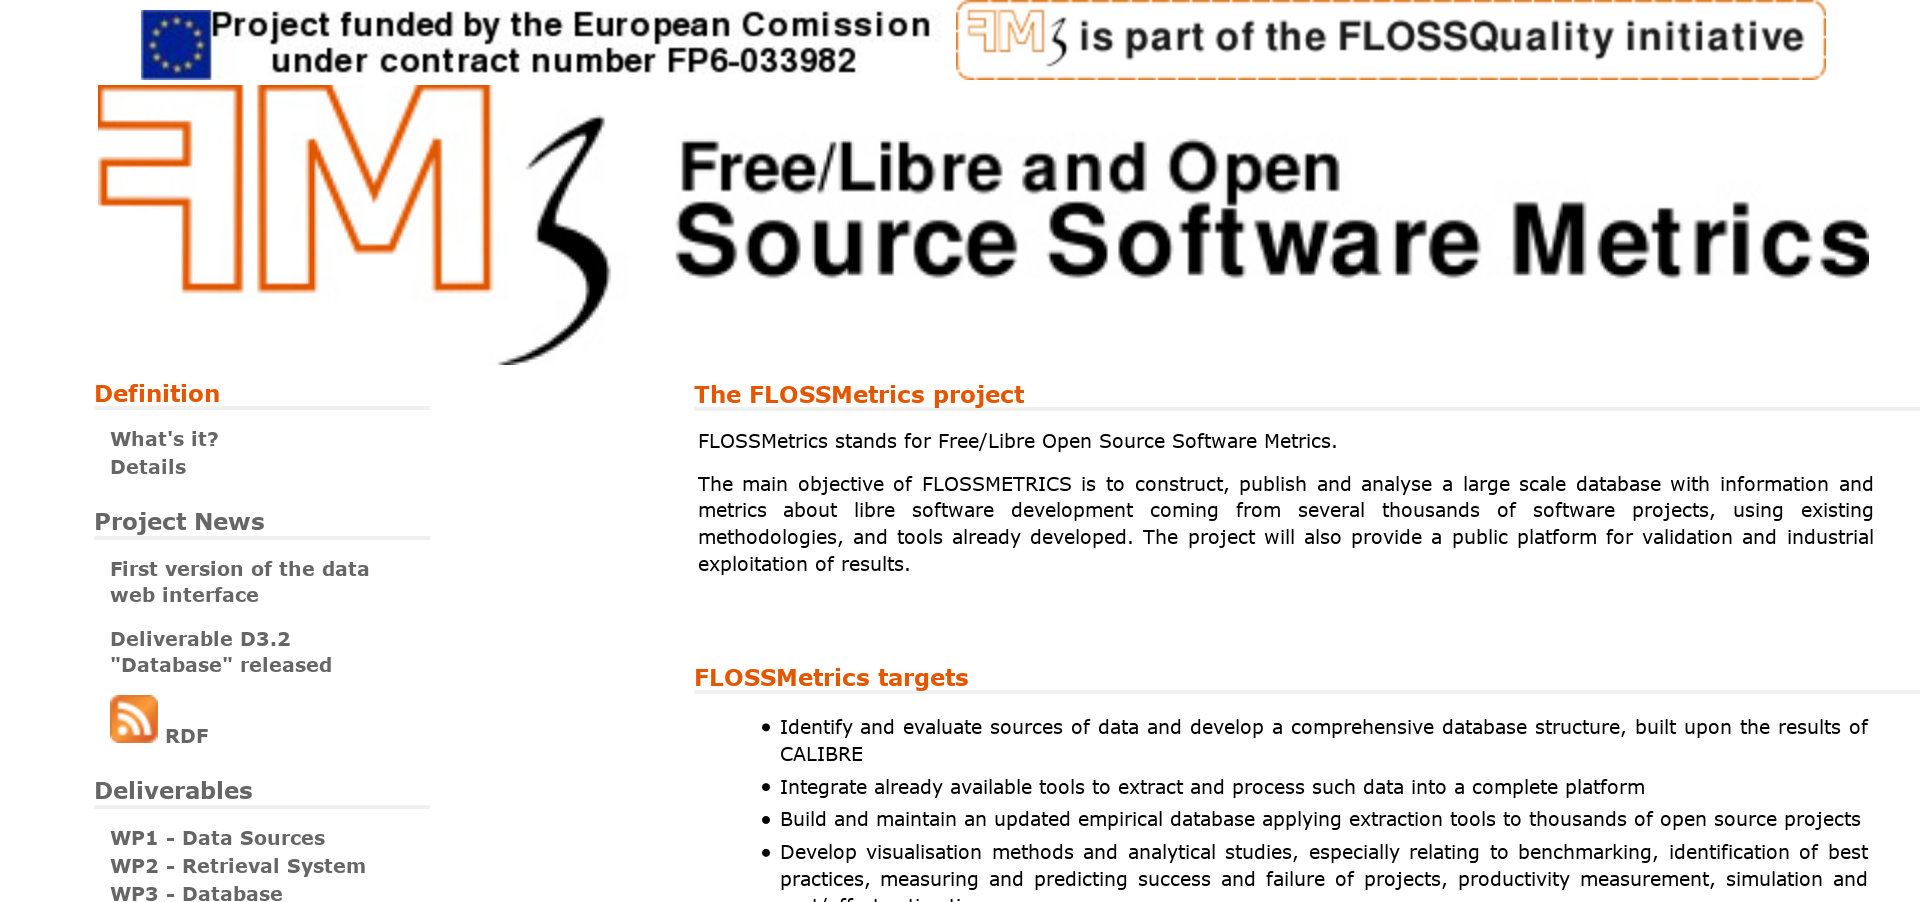
\includegraphics[width=12cm]{figs/flossmetrics}
  \end{center}  
  
\end{frame}

%%-----------------------------------------
\begin{frame}[fragile]
  \frametitle{Funding \& research}

  Funded projects bring resources \\
  They allow for implementing ambitious ideas \\
  They put together interesting teams \\
  
  \begin{center}
    Funded projects may be (very) distracting
  \end{center}  
  
\end{frame}



%%-----------------------------------------
\begin{frame}[fragile]
  \frametitle{Putting data to work (2008-2013)}

  \begin{center}
  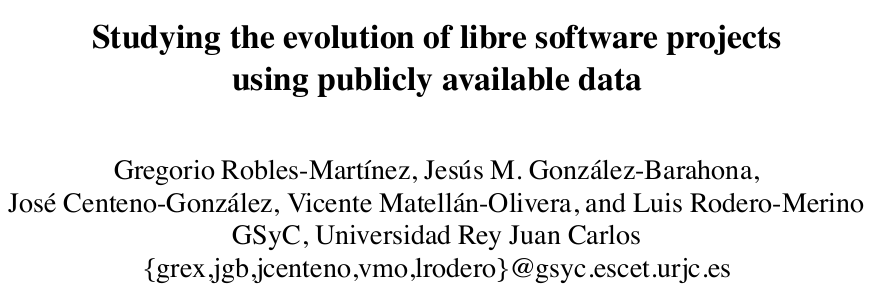
\includegraphics[width=12cm]{figs/evolution-data}
  \end{center}  
  
\end{frame}

%%-----------------------------------------
\begin{frame}[fragile]
  \frametitle{Reproduction studies}

  Reproducing past research is fun \\
  and interesting \\
  and helps to advance the state of the art \\
  It may lead to new lines \\
  
  \begin{center}
    Reproducing is not always easy
  \end{center}  
  
\end{frame}

%%-----------------------------------------
\begin{frame}[fragile]
  \frametitle{Becoming commercial (2010-2013)}

  \begin{center}
  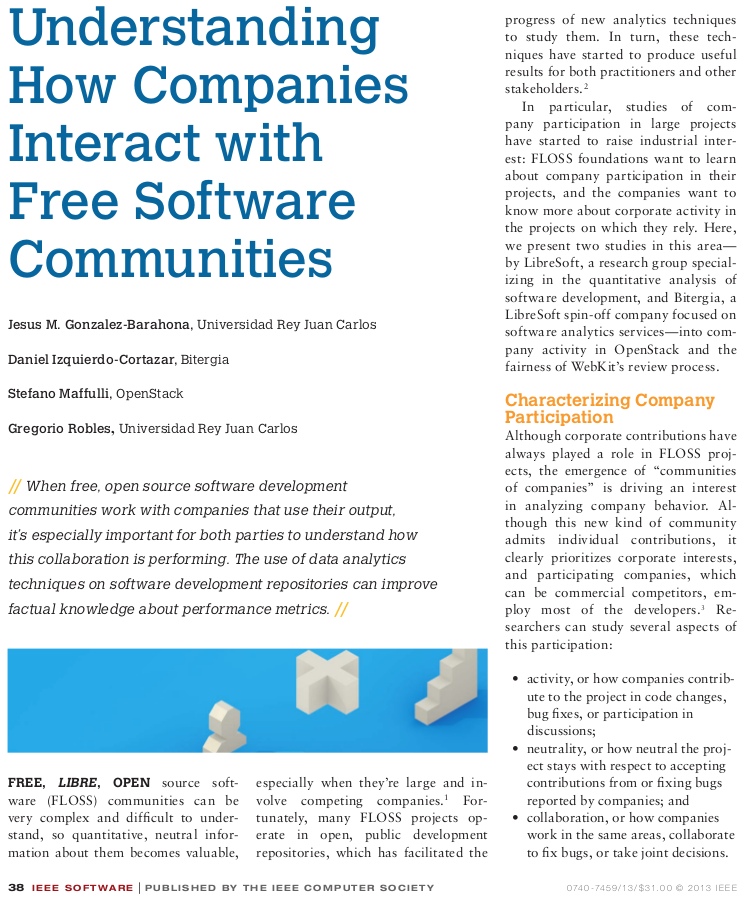
\includegraphics[width=12cm]{figs/software-companies}
  \end{center}  
  
\end{frame}

%%-----------------------------------------
\begin{frame}[fragile]
  \frametitle{Approaching the industry}

  The real world is there, and it's nice \\
  If you can explain a part of it \\
  that will be appreciated \\
  
  \begin{center}
    The real world is dirty, complex, \\
    difficult to understand \\
  \end{center}  
  
\end{frame}

%%-----------------------------------------
\begin{frame}[fragile]
  \frametitle{Mature tooling (2002-2015)}

  \begin{center}
  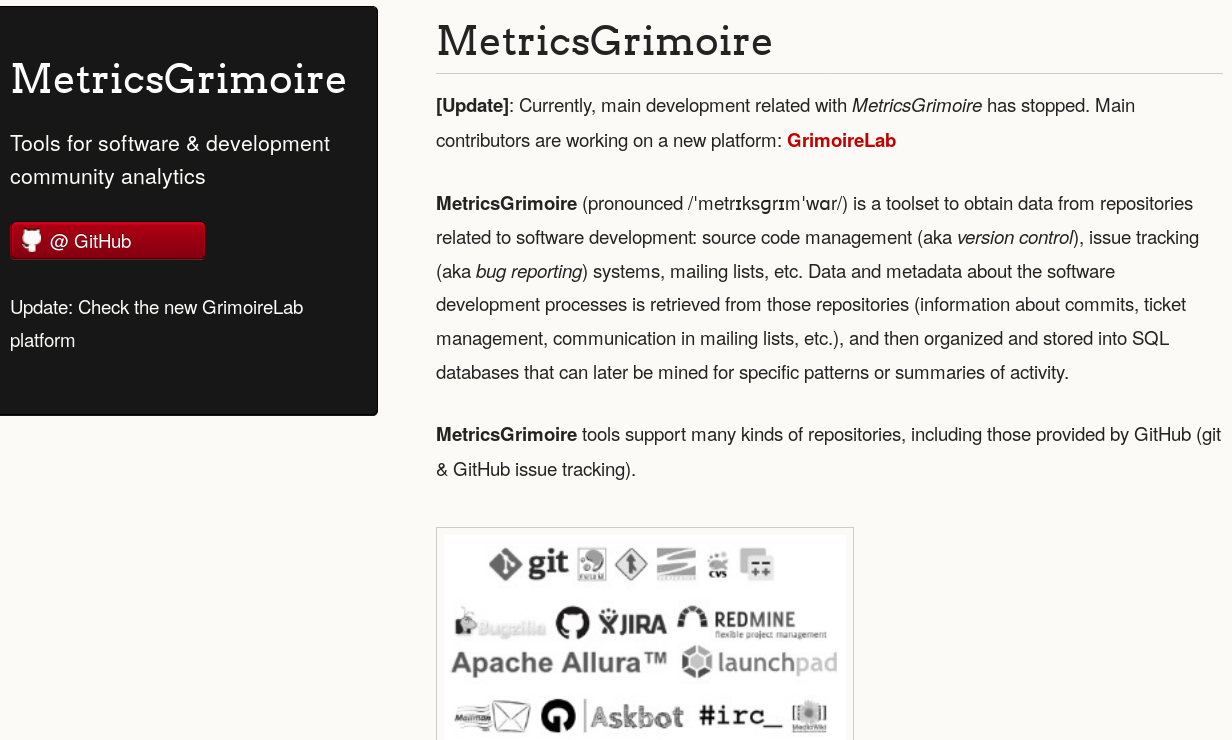
\includegraphics[width=12cm]{figs/metricsgrimoire}
  \end{center}  
  
\end{frame}

%%-----------------------------------------
\begin{frame}[fragile]
  \frametitle{Tools \& research (2)}

  Tools keep you anchored in reality \\
  Tools give you a competitive advantage \\
  Tools let you learn the details \\
  
  \begin{center}
    Tools may be distracting, \\
    difficult to ``convert'' in papers \\
  \end{center}  
  
\end{frame}

%%-----------------------------------------
\begin{frame}[fragile]
  \frametitle{Bitergia (2012-)}

  \begin{center}
  
\includegraphics[width=12cm]{figs/bitergia}
  \end{center}  
  
\end{frame}

%%-----------------------------------------
\begin{frame}[fragile]
  \frametitle{Bitergia (2012-)}

  \begin{center}
  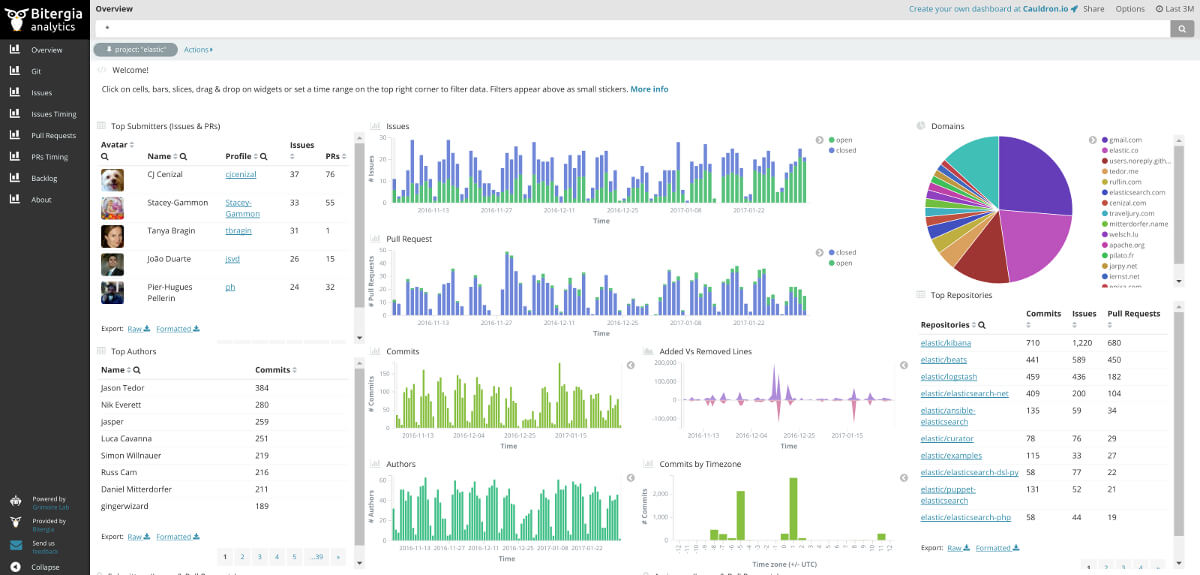
\includegraphics[width=12cm]{figs/bitergia-dashboard}
  \end{center}  
  
\end{frame}

%%-----------------------------------------
\begin{frame}[fragile]
  \frametitle{Bitergia (2012-)}

  \begin{center}
  
\includegraphics[width=10cm]{figs/bitergia-customers}
  \end{center}  
  
\end{frame}

%%-----------------------------------------
\begin{frame}[fragile]
  \frametitle{Bitergia (2012-)}

  \begin{center}
  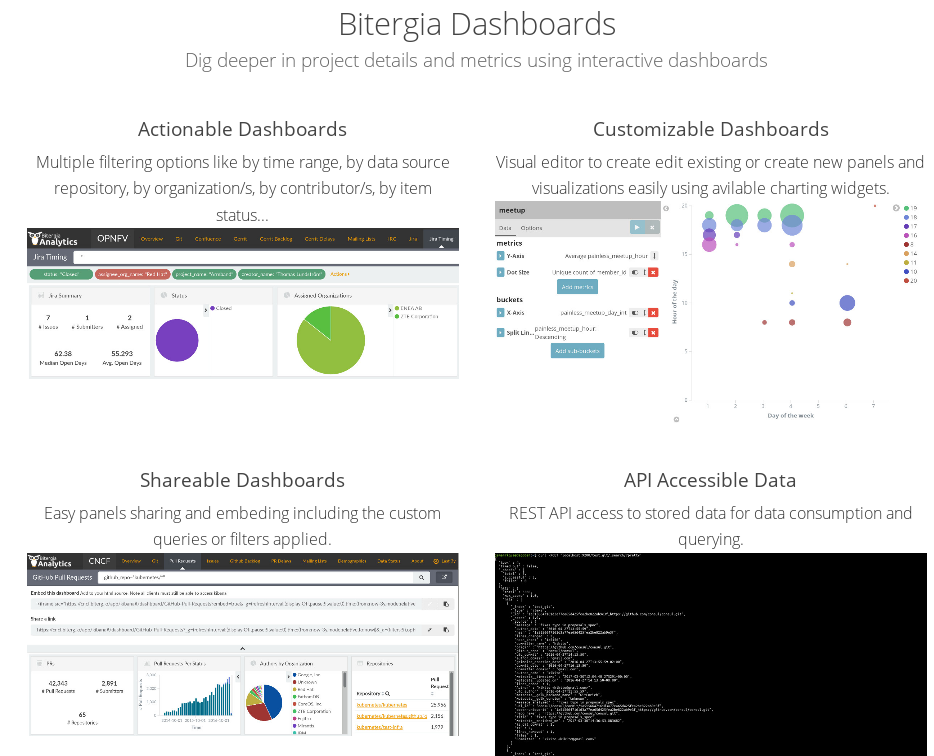
\includegraphics[width=10cm]{figs/bitergia-dashboards}
  \end{center}  
  
\end{frame}

%%-----------------------------------------
\begin{frame}[fragile]
  \frametitle{Bitergia (2012-)}

  \begin{center}
  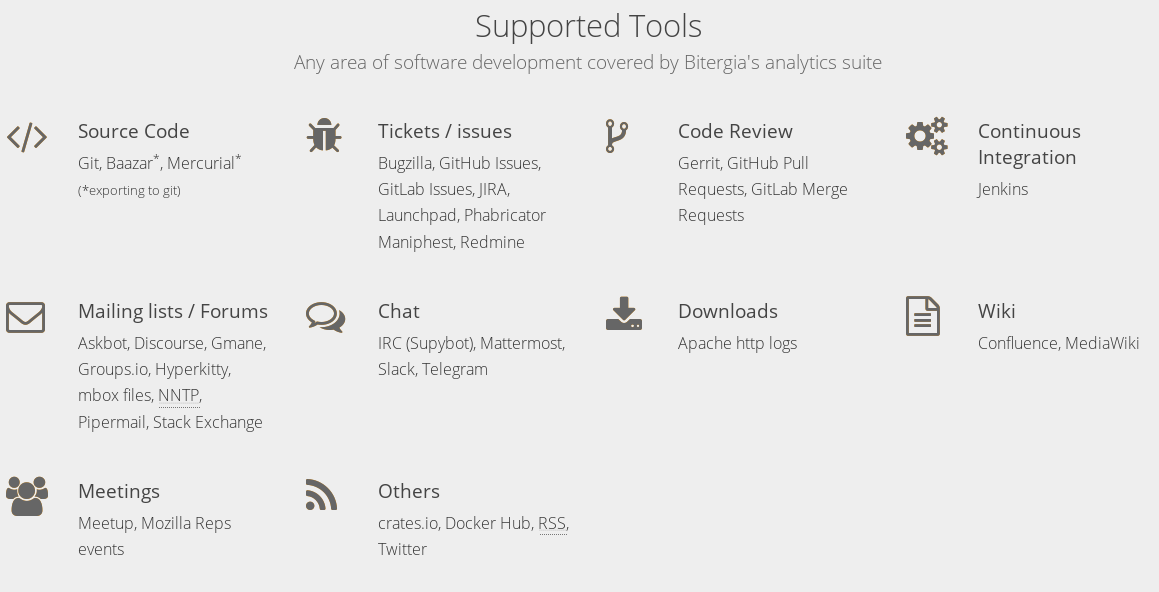
\includegraphics[width=10cm]{figs/bitergia-tools}
  \end{center}  
  
\end{frame}

%%-----------------------------------------
\begin{frame}[fragile]
  \frametitle{Try the stuff yourself!}

  The new Cauldron (still alpha)

  \begin{flushright}
    \url{https://alpha.cauldron.io}
  \end{flushright}

  GrimoireLab

  \begin{flushright}
    \url{https://chaoss.github.io/grimoirelab}
  \end{flushright}
  

\end{frame}

%%-----------------------------------------
\begin{frame}[fragile]
  \frametitle{Starting up}

  Startups are a lot of fun \\
  They link you to reality, \\
  and see a new side of reality \\
  
  \begin{center}
    Startups are a huge sink for your time
  \end{center}  
  
\end{frame}

%%-----------------------------------------
\begin{frame}[fragile]
  \frametitle{Starting}

  We observed a new market, but,

  \begin{flushright}
  how deep it is? \\
  what exactly does it want? \\
  how to reach it? \\
  how to fund the process? \\
  \end{flushright}
  
\end{frame}

%%-----------------------------------------
\begin{frame}[fragile]
  \frametitle{Our approach}

  Small team \\
  Our own money \\
  Organic growth \\
  (growing on customers) \\
  word of mouth \\
  
\end{frame}

%%-----------------------------------------
\begin{frame}[fragile]
  \frametitle{Scaling up}

  Bring expertise in \\
  Learning user needs \\
  Bussiness development is fundamental \\
  New marketing approaches \\
  Dealing with quickly changing tech \\
  
\end{frame}

%%-----------------------------------------
\begin{frame}[fragile]
  \frametitle{From academia to industry}

  In the end, a single metric: \\
  time until all cash is burned \\
  \vspace{1cm}
  Talks are different \\
  Tools are different \\
  Customers are fundamental \\
\end{frame}

%%-----------------------------------------
\begin{frame}[fragile]
  \frametitle{From academia to industry (and back)}

  You gain a lot of unique expertise \\
  You learn what matters in the industry \\
  You learn to appreciate the importance of details \\
  \vspace{1cm}
  \begin{flushright}
    You learn what is
    ``providing value''
  \end{flushright}
\end{frame}

%%-----------------------------------------
%%-----------------------------------------
\section{Summary}


%%-----------------------------------------
\begin{frame}[fragile]

  \begin{center}
  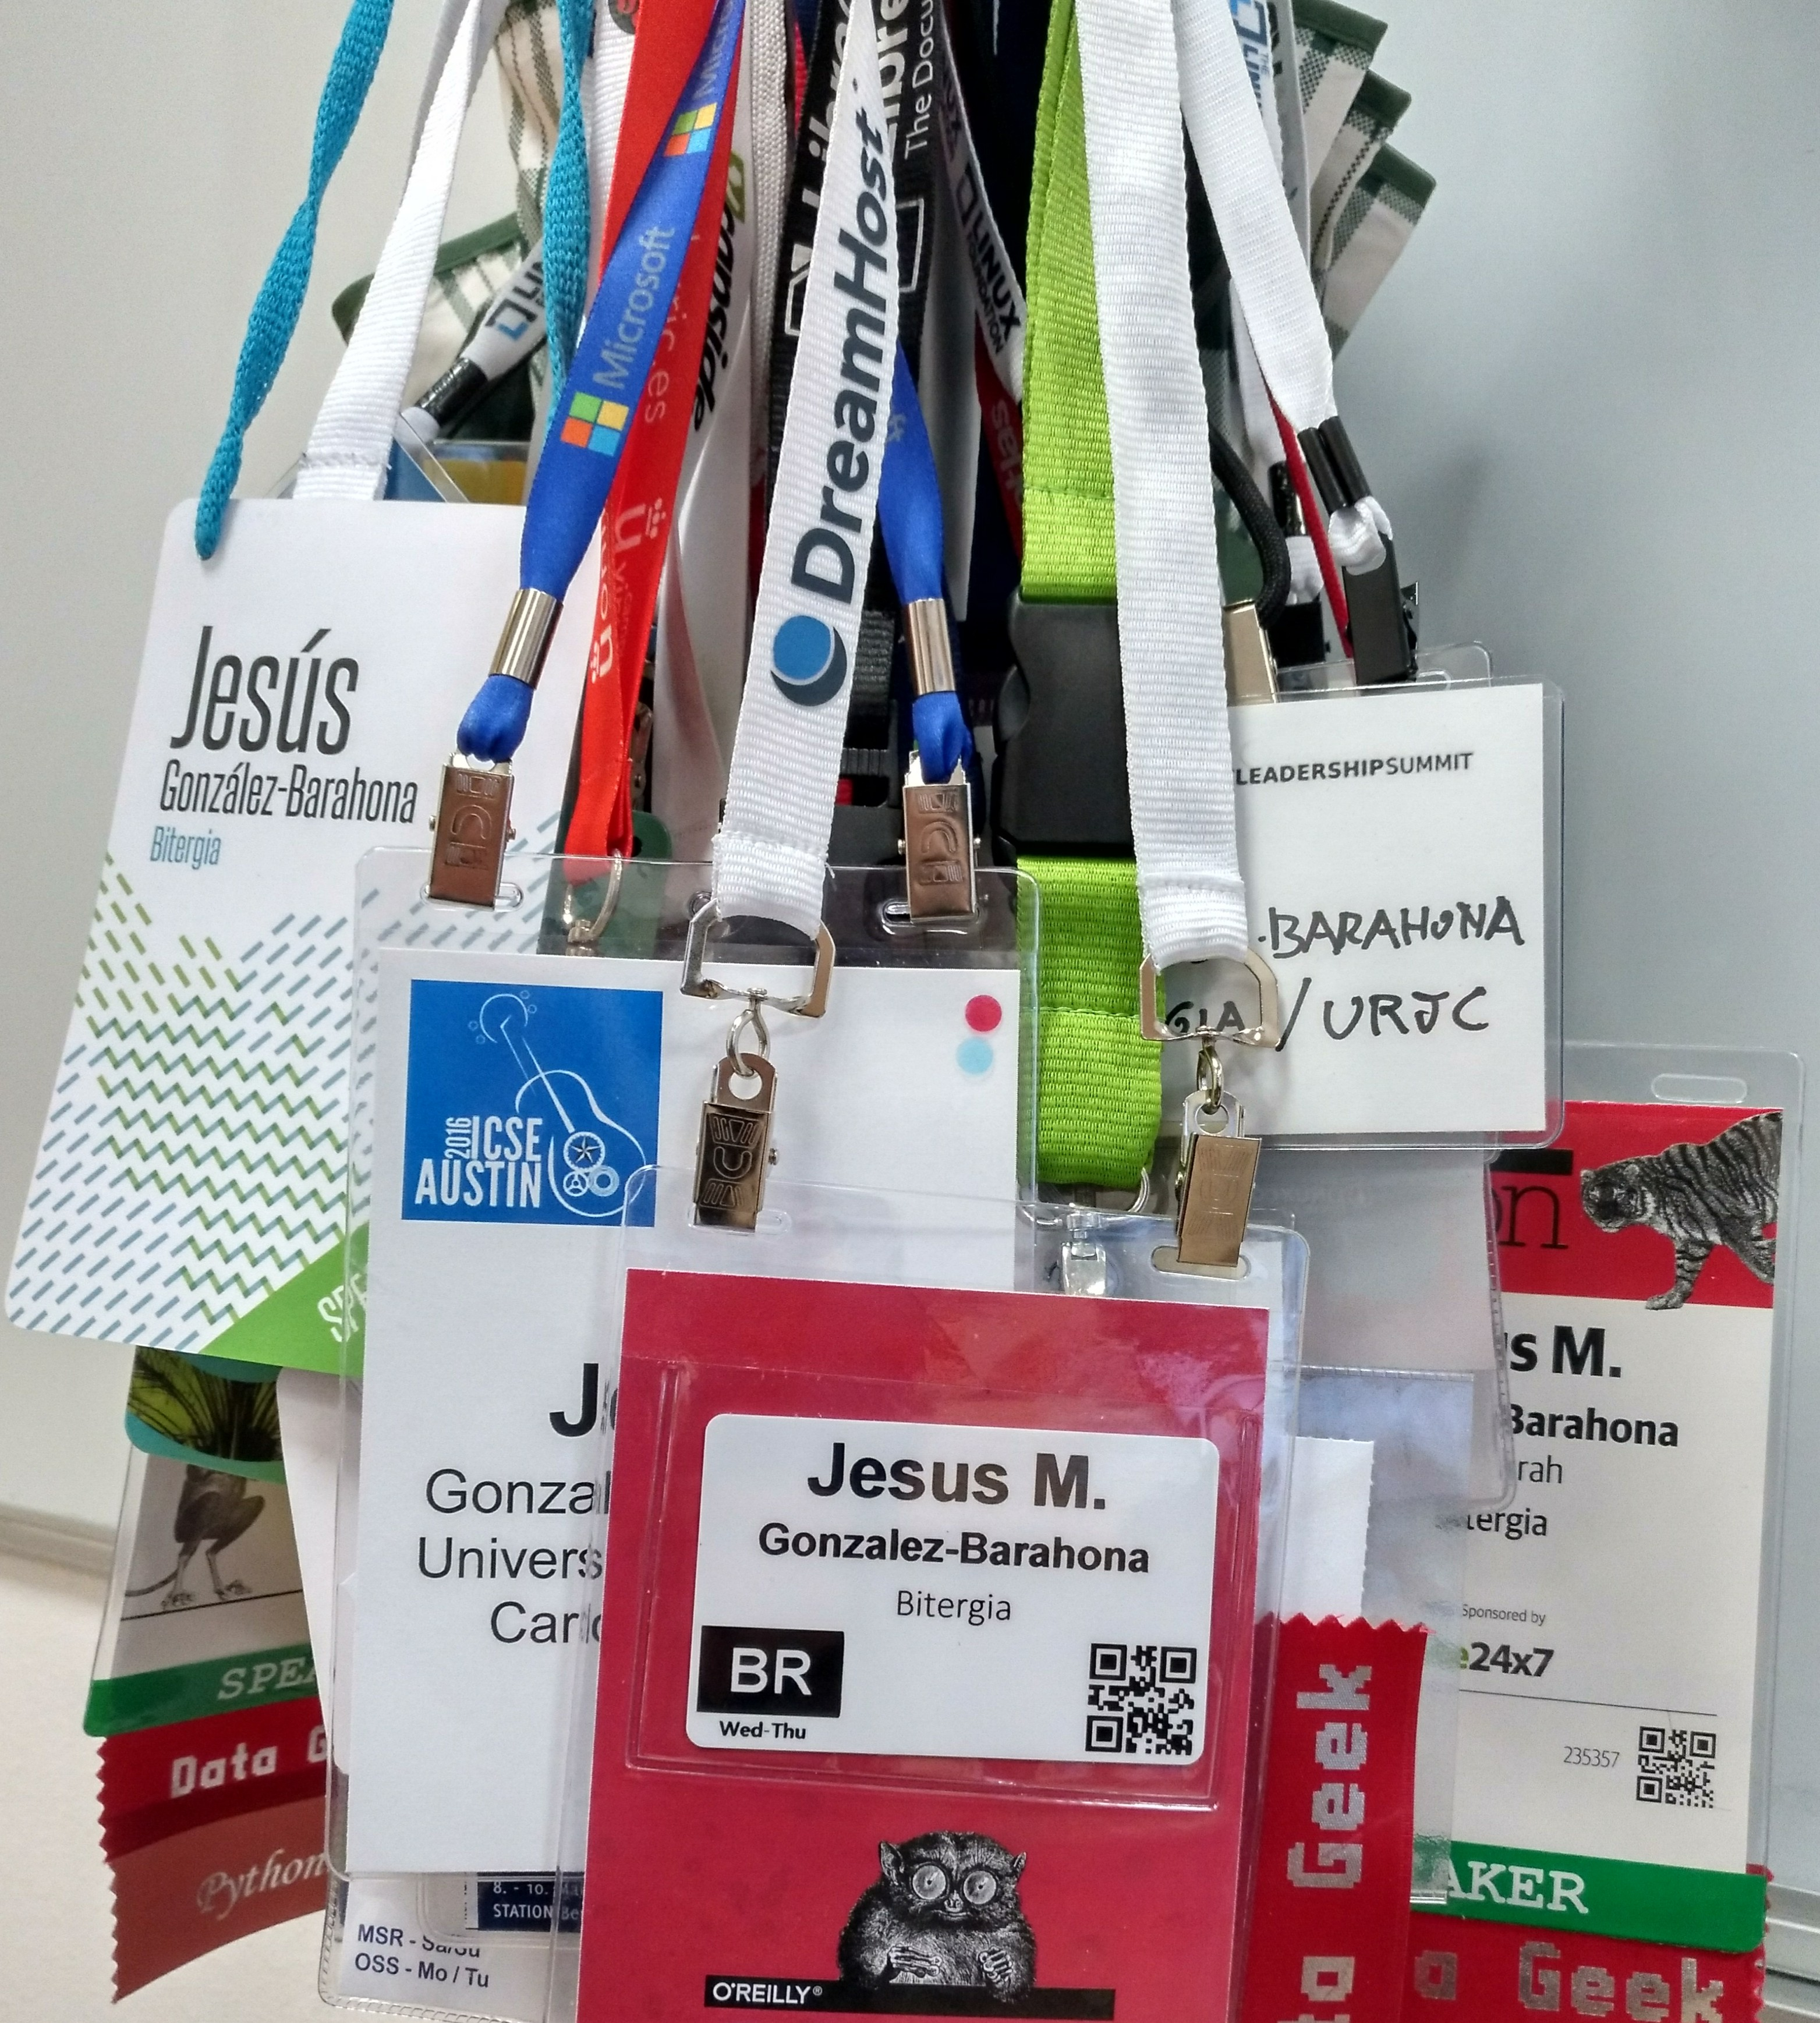
\includegraphics[width=10cm]{figs/badges}
  \end{center}  
  
\end{frame}

%%-----------------------------------------
\begin{frame}[fragile]

  \begin{center}
  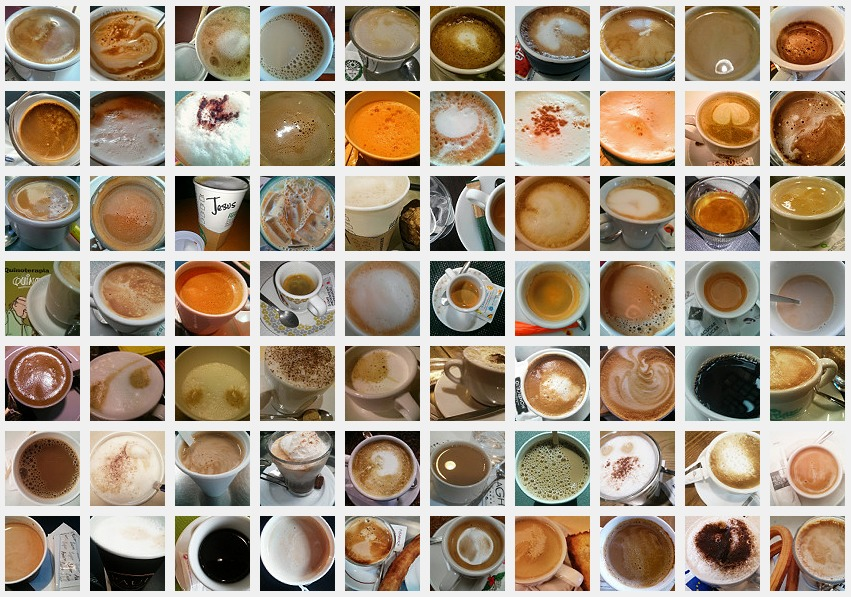
\includegraphics[width=11cm]{figs/coffees}
  \end{center}  
  
\end{frame}

%%-----------------------------------------
\begin{frame}[fragile]

  \begin{center}
    {\em \large
      There is fine line \\
      between being academic \\
      and being commercial \\
      (for you) \\
    }
  \end{center}  
  
\end{frame}

%%-----------------------------------------
\begin{frame}[fragile]

  \begin{center}
    {\em \large
      There is a whole world \\
      of difference \\
      between being academic \\
      and being commercial \\
      (for the rest of the people) \\
    }
  \end{center}  
  
\end{frame}



\frame{
~
\vspace{1cm}

\begin{flushright}


\includegraphics[width=2.2cm]{figs/by-sa}
 \\

\begin{footnotesize}
\copyright 2019 Jesus M. Gonzalez-Barahona. \\

\vspace{.4cm}

Some rights reserverd. This document is distributed under the terms of the Creative Commons License ``Attribution-ShareAlike 4.0'',
available in \\
{\scriptsize \url{http://creativecommons.org/licenses/by-sa/4.0/}} \\

\vspace{.4cm}

This document (including source) is available from
\url{https://github.com/jgbarah/presentations}

\end{footnotesize}
\end{flushright}

}
%%

%\againframe{firstframe}

\end{document}
